\section{Approximations of mean and covariance}

\subsection{a}

Kind of similar to HA2, the key code for 1a is listed here:

\begin{lstlisting}
    % Loop over the number of samples
    for i = 1:numSamples
        % Sample the state vector x from the state density
        x = mvnrnd(mean_x, cov_x)';
        
        % Compute the dual bearing measurement vector y using the state vector x
        y = dualBearingMeasurement(x, s1, s2);
        
        % Add random sample noise to the measurement vector y
        y = y + mvnrnd(zeros(2, 1), cov_r)';
        
        % Store the sample measurement vector y
        samples_y(:, i) = y;
    end

\end{lstlisting}

My \texttt{numSamples} set as 10,000.

\subsection{b}

Here I created a new function \texttt{MeanCovarianceY} based on \texttt{nonLinKFupdate}, since we do not need to update prior of $x$ and its covariance, we only care about the mean and covariance of the measurement.

After modification, acutally its structure is the same with \texttt{nonLinKFprediction}. 

It is not coincidence, for in this question we only care about positions that our state is the same with the measurement. So if we directly input $ h $ and $ R $ to replace the parameters $ f $ and $ Q $ in the function \text{nonLinKFprediction}, it can works.

Here is the table for 2b.
\begin{table}[H]
    \raggedleft
    \begin{tabular}{|l|l|l|}
    \hline
        \textbf{-} & \textbf{EKF\_MEAN} & \textbf{EKF\_cov} \\ \hline
        \textbf{scenario 1} & [0.1974; 1.3734] & [0.0017    0.0015 ;0.0015    0.0060] \\ \hline
        \textbf{scenario 2} & [2.3562; 2.3562] & [0.0500    0.0100 ;0.0100    0.0020] \\ \hline
        \textbf{scenario 3} & [-0.5880, 2.1588] & [0.0092   -0.0111 ; -0.0111    0.0148] \\ \hline
        \textbf{} & ~ & ~ \\ \hline
        \textbf{-} & UKF\_mean & UKF\_cov \\ \hline
        \textbf{scenario 1} & [0.1983 ;1.3743] & [0.0017    0.0015 ;0.0015    0.0059] \\ \hline
        \textbf{scenario 2} & [2.3269; 2.3550] & [0.0600    0.0108 ;0.0108    0.0020] \\ \hline
        \textbf{scenario 3} & [-0.5949; 2.1524] & [0.0099   -0.0112 ; -0.0112    0.0151] \\ \hline
        \textbf{} & ~ & ~ \\ \hline
        \textbf{-} & CKF\_mean & CKF\_cov \\ \hline
        \textbf{scenario 1} & [0.1983 ;1.3743] & [0.0017    0.0015 ;0.0015    0.0059] \\ \hline
        \textbf{scenario 2} & [2.3265; 2.3550] & [0.0566    0.0105 ;0.0105    0.0020] \\ \hline
        \textbf{scenario 3} & [-0.5948; 2.1523] & [0.0097   -0.0112 ; -0.0112    0.0150] \\ \hline
    \end{tabular}
    \caption{Table For Three Densities}
\end{table}

\subsection{c}

\begin{figure}[H]
 \centering
 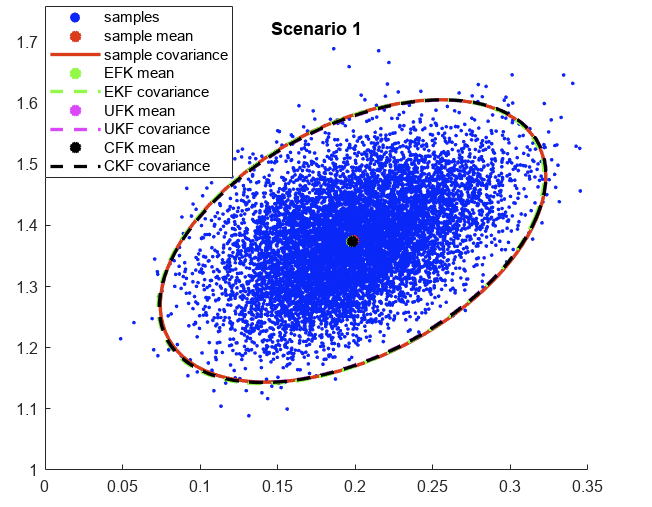
\includegraphics[width=0.7\textwidth]{images/scenario1.png}
 \caption{Density1}
 \label{s1}
\end{figure}
\begin{figure}[H]
 \centering
 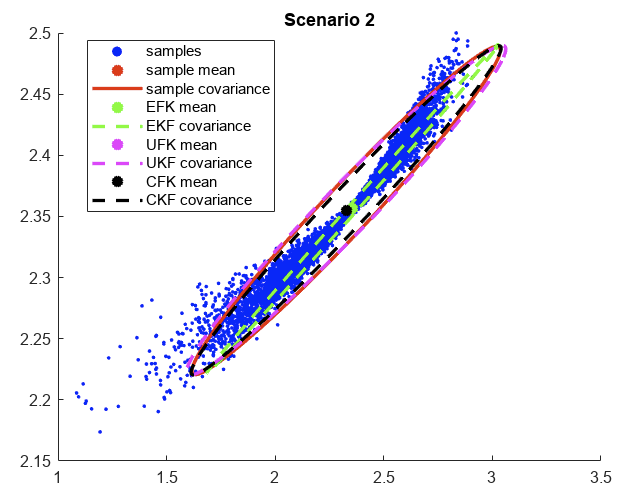
\includegraphics[width=0.7\textwidth]{images/scenario2.png}
 \caption{Density2}
 \label{s2}
\end{figure}
\begin{figure}[H]
 \centering
 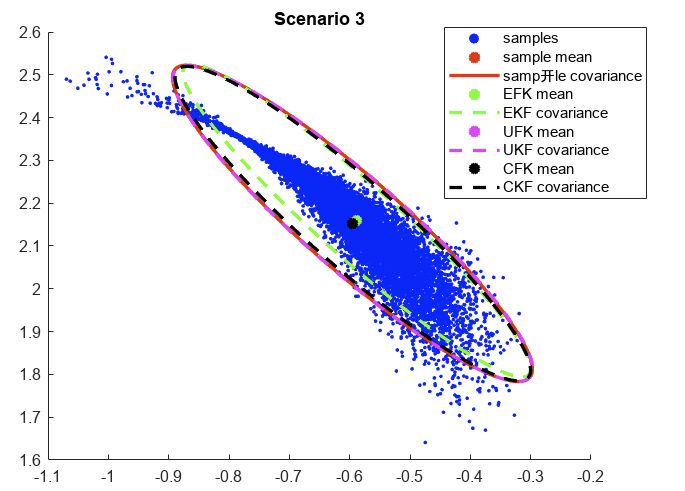
\includegraphics[width=0.7\textwidth]{images/scenario3.png}
 \caption{Density3}
 \label{s3}
\end{figure}

\emph{Note: The covariance curves are drawn by the function \texttt{sigmaEllipse2D} created by myself in previous function, which depicted 3 $ sigma $ curves.}

In three figures, the aprromaxiation methods perform well that their mean and covariance are really close to the sample value.

But for \texttt{EKF} method, it only perform well in figure \ref{s1}, in both 2 and 3, there are different extent of divergences, especially in 2, where its covariance has almost completely shifted away from the curve of sample covariance curve.

\subsection{d}

In all three pictures, the approximate means/covariances are nearly as the same places with the sample mean/covariance. That is because the approximation methods \texttt{UKF, CKF } all fairly useable in nonlinear measurement model.

But for \texttt{EKF} method, it perform much worser in figure \ref{s2} and figure \ref{s3}. That is because the \texttt{EKF} assume the model is linear at the operating point, while in scenario 2 and 3 the model is too nonlinear for it.

UKF and CKF perform always good because it do not set requiements for the model.However, compared to EKF methods, they are more computationally intensive and more expensive to use.

If I were an engineer, I would definitely use the EKF method without a doubt in a very linear situation, because it is faster and cheaper. For mildly nonlinear cases, the EKF can be considered according to the actual needs, like in Figure \ref{s3}, where the EKF can be used if the accuracy is not too demanding. But for extreme nonlinear cases, as in Figure \ref{s2}, I would not choose the EKF method.